\documentclass[a4paper, 12pt]{article}

\usepackage{hyperref}
\usepackage[warn]{mathtext}
\usepackage[utf8]{inputenc}
\usepackage[T2A]{fontenc}
\usepackage[english,russian]{babel}
\usepackage{multirow}
\usepackage{float}
\restylefloat{table}
\usepackage{amsmath,amsfonts,amssymb,amsthm,mathtools}
\usepackage{indentfirst}
\DeclareSymbolFont{T2Aletters}{T2A}{cmr}{m}{it}
\usepackage{ gensymb }
\mathtoolsset{showonlyrefs=true}
\usepackage{euscript}
\usepackage{mathrsfs}
\usepackage[left=2cm,right=2cm,top=2cm,bottom=2cm]{geometry}
\usepackage{graphicx}
\usepackage{wrapfig}
\usepackage[rgb]{xcolor}
\hypersetup{
	colorlinks=true,
	urlcolor=blue
}
\usepackage{tikz}

\title{Лабораторная работа}
\author{Гисич Арсений Б03-102}
\date{2023}

\begin{document}

	\begin{center}
		{\large МОСКОВСКИЙ ФИЗИКО-ТЕХНИЧЕСКИЙ ИНСТИТУТ (НАЦИОНАЛЬНЫЙ ИССЛЕДОВАТЕЛЬСКИЙ УНИВЕРСИТЕТ)}
	\end{center}
	\vspace{5 cm}
	{\Large
		\begin{center}
			{\bf Лабораторная работа 4.5.3}\\[0.2 cm]
			Сканирующий интерферометр
		\end{center}
	}
	\vspace{4 cm}
	\begin{flushright}
		{\Large Выполнили: \\
			\vspace{0.2 cm}
			Айрапетян Микаел \\
			Гисич Арсений \\
			\vspace{0.2 cm}
			Б03-102 \\}
	\end{flushright}
	\vspace{8 cm}
	\begin{center}
		Долгопрудный\\[0.1 cm]
		2023
	\end{center}
\thispagestyle{empty}

\section{Аннотация}

В данной работе были изучены устройство и работа газового лазера непрерывного действия, спектральные характеристики лазерного излучения, а также устройство и принцип действия сканирующего интерферометра Фабри-Перо.

\section{Методика измерений}

Для генерирующихся в лазере мод:
\begin{equation} \label{eq:rez_modes}
2L = m\lambda
\end{equation}
\noindent где $L$ --- длина резонатора лазера

Условие резонанса для интерферометра:
\begin{equation} \label{eq:int_modes}
2l = m\lambda
\end{equation}
\noindent где $l$ --- база интерферометра

Собственные моды интерферометра отличаются по частоте на величину:
\begin{equation} \label{eq:nu_dif}
\Delta \nu = \frac{c}{2L}
\end{equation}

Дисперсионная область $\Delta \nu$ в единицах $\lambda$:
\begin{equation} \label{eq:disp}
\Delta \lambda_{\text{СИ}} = \frac{\lambda}{m}= \frac{\lambda^2}{2l}
\end{equation}

Разрешающая способность интерферометра Фабри-Перо:
\begin{equation} \label{eq:resolution}
R = \frac{\lambda}{\delta{\lambda}}
\end{equation}

Разрешающая способность интерферометра Фабри-Перо зависит от длины интерферометра $l$ и коэффициента отражения зеркал $r$:
\begin{equation} \label{eq:refl}
R = \frac{2\pi l}{\lambda (1-r)}
\end{equation}

\begin{figure}[H]
	\centering
	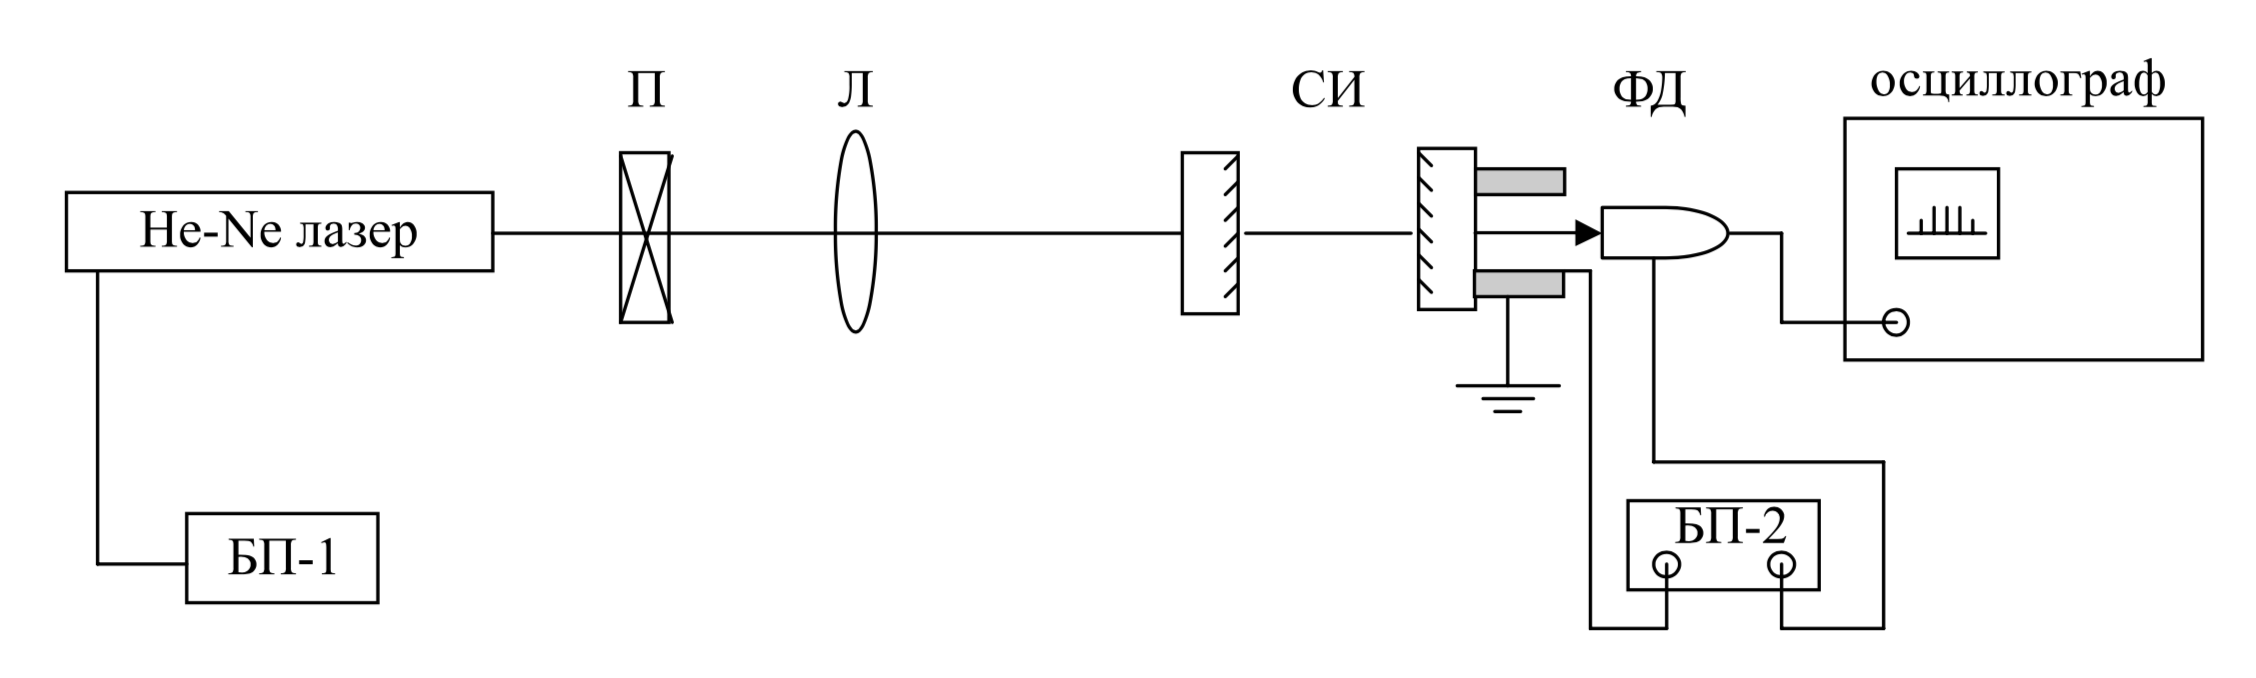
\includegraphics[width=0.9\textwidth]{1.png}
	\caption{Схема установки для исследования спектрального состава излучения лазера}
	\label{fig:ust}
\end{figure}

\begin{figure}[H]
	\centering
	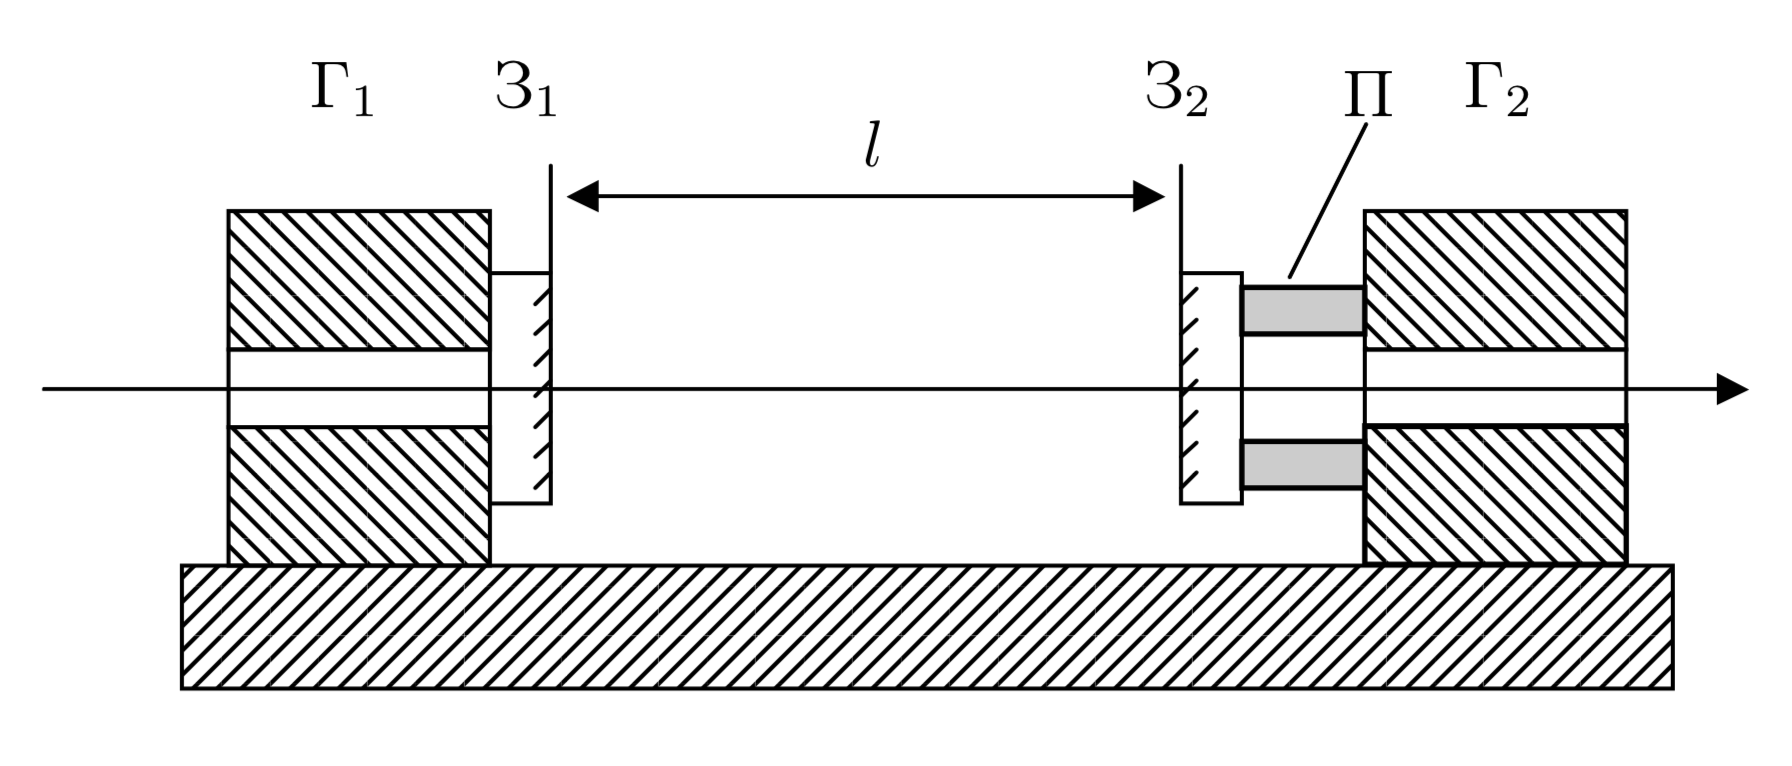
\includegraphics[width=0.8\textwidth]{2.png}
	\caption{Устройство сканирующего интерферометра}
	\label{fig:rez}
\end{figure}

\begin{figure}[H]
	\centering
	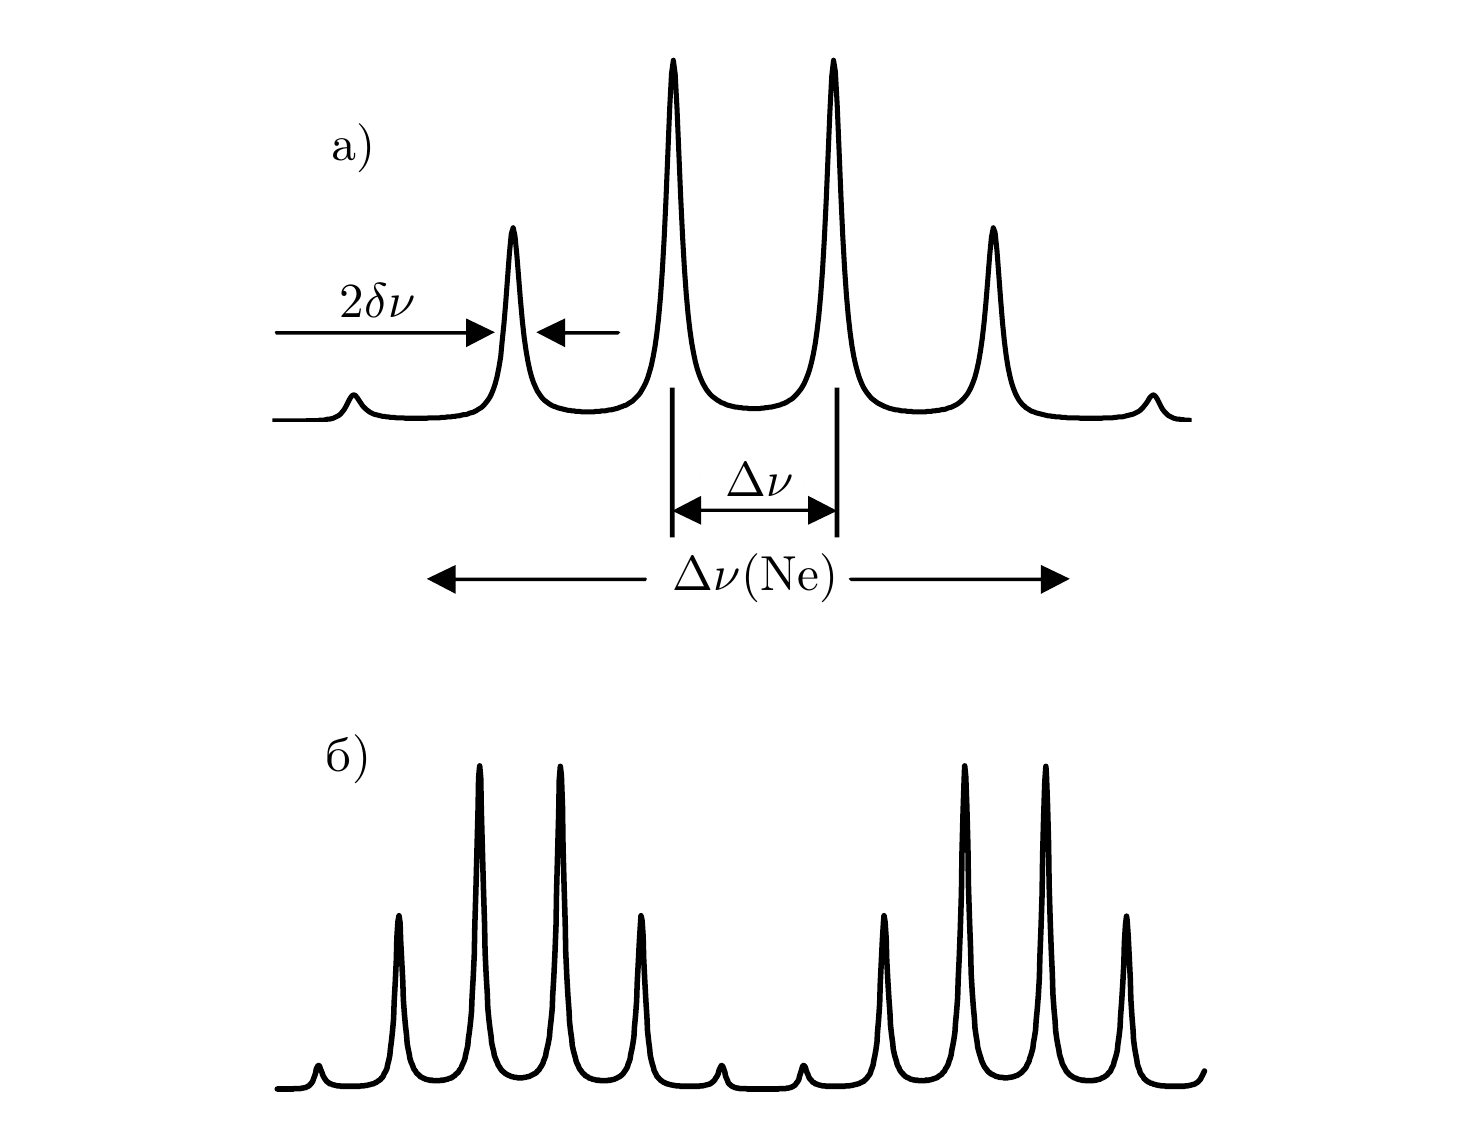
\includegraphics[width=0.8\textwidth]{3.png}
	\caption{Характерные осциллограммы: а) при небольшой амплитуде колебаний зеркала \newline ( $\leqslant \lambda/2$), б) при амплитуде колебаний, превышающей $\lambda/2$}
	\label{fig:osc}
\end{figure}
 	
\section{Используемое оборудование}

\begin{enumerate}
    \item He--Ne-лазер с блоком питания;
    \item Сканирующий интерферометр Фабри--Перо;
    \item Поляроид;
    \item Пластинка $\lambda/4$;
    \item Линза;
    \item Фотодиод;
    \item Электронный осциллограф.
\end{enumerate}

\section{Результаты измерений и обработка данных}

Параметры установки:
\begin{description}
\item{} $\lambda =6328~\text{\AA}$
\item{} $L = 65~см$
\item{} $l = 9~см$
\end{description}

Проведём настройку оптической системы. Для этого сначала уберём линзу из луча с помощью поперечных салазок. Совместим прямой и отражённый пучки, вращая винты на первом по ходу луча зеркале интерферометра. Затем винтами второго зеркала совместим пятна на первом зеркале.

Настроим поляризационную развязку. Вращая пластинку $\lambda/4$ погасим отражённый луч.

Введём линзу в пучок для уменьшения расходимости пучка и усиления сигнала. Перемещая фотодиод, получим на экране осциллограмму как на рис.~\ref{fig:osc}. Добьёмся максимального сигнала. Подберём напряжение на пьезокристалле, при котором на экране будет укладываться 1--2 контура.

\begin{figure}[H]
\begin{center}
    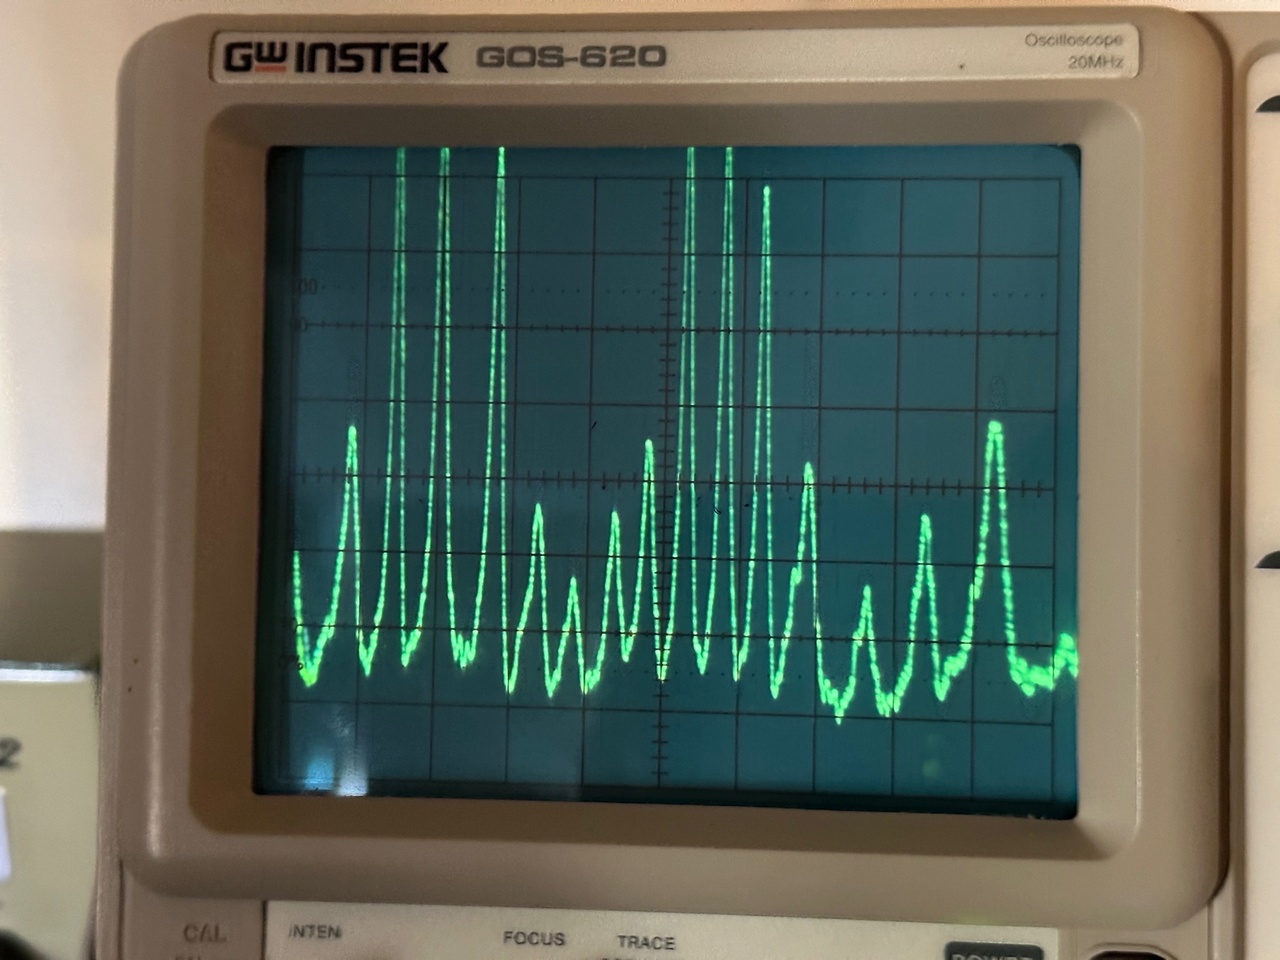
\includegraphics[width=0.6\textwidth]{oscma.jpg}
\end{center}
\caption{Полученная осциллограмма}
\label{fig:oscma}
\end{figure}

По формуле \eqref{eq:nu_dif} рассчитаем межмодовое расстояние резонатора: 
$$\nu_{m+1} - \nu_m = \frac{c}{2L} = 230~МГц.$$

По формуле \eqref{eq:disp} рассчитаем дисперсионную область сканирующего интерферометра в единицах $\nu$ и $\lambda$:
$$\Delta{\lambda_{СИ}} = \frac{\lambda^2}{2l} = 0,02~\text{\r{A}}.$$
$$\Delta{\nu_{СИ}} = \frac{c}{2l} = 1,6~\cdot~10^9~Гц$$

Сосчитав число промежутков между модами на экране, оценим видимую ширину спектральной линии неона. На рис.~\ref{fig:oscma} видно 7 промежутков, значит $\Delta{\lambda(Ne)} = 7 \cdot 230 = 1610~МГц.$

Полагая, что ширина спектральной линии обусловлена эффектом Доплера и что видимая ширина линии неона порядка полуширины доплеровского контура ($\Delta{\lambda(Ne)} \sim \Delta{\lambda_D}$), оценим среднюю скорость атомов неона $v_x$: 
$$\frac{\Delta{\lambda_D}}{2\lambda} \approx \frac{v_x}{c} \Rightarrow v_x \approx 474~м/с.$$
Газокинетическую температуру $T$ в разряде найдём из распределения Максвелла:
$$\frac{1}{2} = \exp{\left(-\frac{m(Ne) v_x^2}{2 k T}\right)} \Rightarrow \ln{2} = \frac{m(Ne) v_x^2}{2 k T} \Rightarrow T = 399~K.$$

Сравнив ширину отдельной моды на полувысоте с межмодовым расстоянием, оценим разрешение сканирующего интерферометра $\delta{\lambda} = 8~\cdot~10^{-4}~\text{\r{A}}$.  По формуле \eqref{eq:resolution} оценим разрешающую способность $R = 8~\cdot~10^{6}$.

По формуле \eqref{eq:refl} оценим коэффициент отражения зеркал интерферометра $r = 0,89$.

\section{Обсуждение результатов и выводы}

В данной работе был исследован доплеровский контур спектральной линии излучения лазера; было определено межмодовое расстояние и приборная ширина отдельной моды излучения лазера; оценена газокинетическая температура в разряде; были рассчитаны дисперсионная область, разрешающая способность и коэффициент отражения зеркал сканирующего интерферометра.

\end{document}
